\chapter{Dise\~no metodol\'ogico}
\label{sec:diseno}
\section{Hip\'otesis}
¿Es posible desarrollar un prototipo capaz de identificar posibles clientes de una empresa a trav\'es de sus h\'abitos en la plataforma FourSquare?
\section{Tipo de investigaci\'on}
Esta investigaci\'on tomar\'a un enfoque cuantitativo.
\section{Poblaci\'on}
Usuarios de FourSquare en la ciudad de Pereira que encajen con el perfil seleccionado
\section{Muestra}
Basado en una muestreo aleatorio simple, con un nivel de confianza del 95\%, se obtiene una muestra de 457 cuentas que representan la poblaci\'on de usuarios de FourSquare en Pereira.
\section{Variables}
Las variables ser\'an las siguientes:
\begin{itemize}
\item Cantidad de usuarios de FourSquare de Pereira.
\item Cantidad de registros procesados.
\item Cantidad de usuarios reconocidos.
\item Cantidad de usuarios reconocidos exitosamente.
\item Tiempo que tarda en ejecutarse la tarea.
\end{itemize}
\section{Dise\~no de instrumentos}
La \ref{fig:instrumentos} contien el instrumento dise\~nado para la toma de datos.
\begin{figure}[h]
\begin{center}
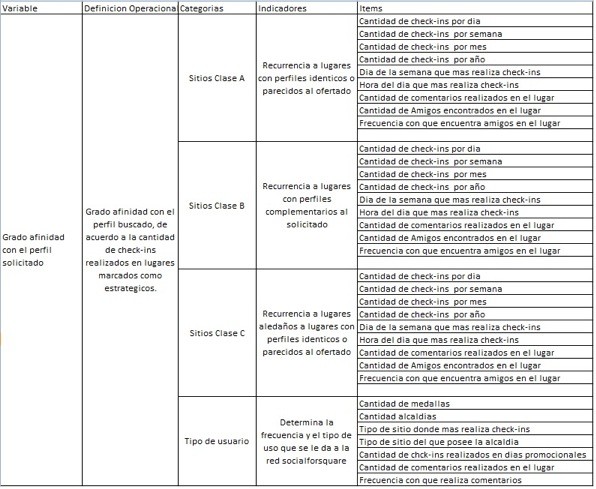
\includegraphics[scale=0.7]{./instrumentos.png}
\end{center}
{\caption{Tabla de dise\~no de instrumentos}\label{fig:instrumentos}}
\end{figure}
\clearpage
\pagebreak